\item \textbf{{[}IJC/PRELIM/9597/2018/P1/Q3{]} }

A binary tree structure is used to store the names of animals in the
Singapore Zoo. Each animal\textquoteright s name is unique. The binary
tree abstract data type (ADT) has commands to create a new tree, add
data items and print the tree.

The sequence of commands:

\noindent %
\noindent\begin{minipage}[t]{1\columnwidth}%
\texttt{CreateTree() }

\texttt{AddToTree('Tiger') }

\texttt{AddToTree('Lemur') }

\texttt{AddToTree('Bat') }

\texttt{AddToTree('Yak') }

\texttt{AddToTree('Ostrich') }

\texttt{AddToTree('Raccoon') }

\texttt{AddToTree('Macaw')}

\texttt{AddToTree('Zebra')}%
\end{minipage}

would create the following binary tree:
\begin{center}
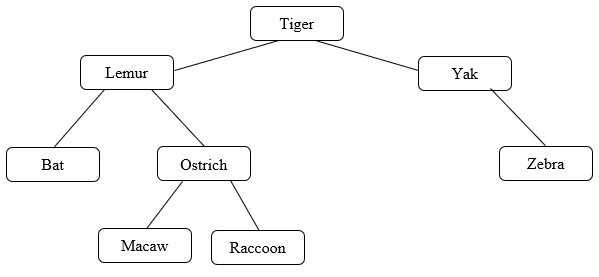
\includegraphics[width=0.5\paperwidth]{C:/Users/Admin/Desktop/Github/question_bank/LyX/static/img/9597-IJC-2018-P1-Q3}
\par\end{center}

The program to implement the ADT will use the classes Tree and Node
designed as follows:
\begin{center}
\begin{tabular}{|l|}
\hline 
\texttt{\hspace{0.25\columnwidth}Tree}\tabularnewline
\hline 
\texttt{thisTree : ARRAY of Node}\tabularnewline
\texttt{root : INTEGER}\tabularnewline
\hline 
\texttt{constructor()}\tabularnewline
\texttt{add(newItem)}\tabularnewline
\texttt{print()}\tabularnewline
\tabularnewline
\tabularnewline
\tabularnewline
\hline 
\end{tabular}%
\begin{tabular}{|l|}
\hline 
\texttt{\hspace{0.25\columnwidth}Node}\tabularnewline
\hline 
\texttt{data : STRING}\tabularnewline
\texttt{leftPtr : INTEGER}\tabularnewline
\texttt{rightPtr : INTEGER }\tabularnewline
\hline 
\texttt{constructor()}\tabularnewline
\texttt{setData(s : STRING)}\tabularnewline
\texttt{setLeftPtr(x : INTEGER)}\tabularnewline
\texttt{setLeftPtr(x : INTEGER)}\tabularnewline
\texttt{getData() : STRING}\tabularnewline
\texttt{getLeftPtr() : INTEGER }\tabularnewline
\texttt{getRightPtr() : INTEGER}\tabularnewline
\hline 
\end{tabular}
\par\end{center}

The program code will do the following:
\begin{itemize}
\item Create a new tree, which has: 
\begin{itemize}
\item no nodes 
\item the root set to --1 
\end{itemize}
\item Use the root as a pointer to the first node in the tree
\item Add a new node to the tree in the appropriate position. The left and
right pointers of this node should have the initial value of --1. 
\item Use the \texttt{print()} method to output, for each node, in array
order: 
\begin{itemize}
\item the data item
\item the left pointer 
\item the right pointer.
\end{itemize}
\end{itemize}

\subsection*{Task 3.1 }

Write program code to define the classes \texttt{Tree} and \texttt{Node}.

\subsection*{Evidence 5}

Your program code. \hfill{}{[}26{]}

\subsection*{Task 3.2}

The program is to be tested. Write a sequence of program statements
to:
\begin{itemize}
\item create a new tree 
\item add the data items as shown in the sequence of commands on the previous
page 
\item print the array contents.
\end{itemize}
Execute your program to test it.

\subsection*{Evidence 6 }

Your program code.

Screenshot of test run. \hfill{}{[}3{]}

\subsection*{Task 3.3 }

A method \texttt{postOrderTraversal()} is to be added. This left-to-right
post-order traversal outputs the data stored in the child nodes before
outputting the data stored in the root node. 

Write program code to:
\begin{itemize}
\item implement this method
\item Test the program code with the data from Task 3.2.
\end{itemize}

\subsection*{Evidence 7 }

Your program code. 

Screenshot of test run.\hfill{} {[}7{]}